\subsection{Hopfield Network}

\subsubsection{Implementation Example: Optical Information Processing}
In paper from D.Psaltis and N.Farhat(1985) \cite{optical_processing}, thresholding and feedback properties from Hopfield model was used in implementation of an optical system that processes optical information.

Enhanced error-correcting capability is one important outcome which is benefited from Nonlinearity of Hopfield model. With $M$ words of each binary vector $v_i$ with length of N bits, matrix $T_{ij}$ represents a storage of information. Matrix $T_{ij}$ gets multiplied by a stored binary vector $v'_i$ results in a \texttt{pseudoeigensystem} if $N$ is sufficiently larger than $M$. This indicated that the output vector $v''_i$ equals the input.

Supposed nonlinear iterative procedural experiments of certain number of known bits $N_1$ and the rest bits set to zero inside total of $N$ bits long vector were addressed to discover under what conditions the number of correct bits $N_2$ in output will be higher than $N_1$. A SNR(signal-to-noise ratio) equation which consists ratio of the expected value to the standard deviation on the same output vector, was used. As the Hopfield model has studied on the convergence property with respect to asynchronous operations, insensitivity to imperfections(nonuniformities, exact form of the threshold operation and errors in $T_{ij}$ matrix) and correct convergence obtained with thresholded $T_{ij}$. These all become most desired properties in optical implementation. Detailed optical implementation with 2D inputs was presented which was based on spatial-frequency multiplexing. Methods using Fourier transform, transmitting amplitude(weighted sum) and integral of the product of the input images were introduced in such an implementation. The robustness of a such system with nonlinear feedback becomes the most important feature.
As a conclusion, the implementation with the capabilities and limitations of optical techniques matches excellently with the Hopfield model that requires global, linear operations and local, point nonlinearities in a fully interconnected optical system.

\subsubsection{Memory Capacity with Modification: \\ replacing sigmoid neuron with a nonmonotonic neuron}
In paper from S.Yoshizawa, M.Morita and S.Amari(1992) \cite{capacity_of_nonmonotonic_model} it started with introduction of a new method by replacing sigmoid neuron with a nonmonotonic neuron and discussed theorectically on potential of absolute capacity(the maximum number of randomly generated patterns which are memorized as the equilibria of the network with the correlation-type connection weights) to be of order $n$ (nearly equal to $0.4n$).

Previous memory capacities were briefly introduced that Hopfield(1982) model's associative memory capacity is $0.15n$, the proven result of absolute capacity is asymptotically $ \frac{n}{2\log{n}} $ (from McEliece, Posner, Rodemich, \& Venkatesh, 1987; Weisbuch, 1985), and relative capacity(recalling process) is about 0.14n(with admission of small percent of errors) with replica method, but about $0.16n$ with a simply approximation method from respectively two different research work.

Various research suggestions were mentioned though all failed to deal completely with flaws of the conventional model, that both absolute and relative capacities are too small as well as the existence of large number of spurious memories. With a nonmonotonic neuron the result turned to be $0.4n$ for the absolute capacity which is even greater than relative capacity while the spurious memory disappeared.

With conventional neuron, memorized pattern is unstable, whereas a basin of attraction around memorized pattern was shown with nonmonotonic neuron by replacing sigmoid function with a nonmonotonic output function \textit{figure \ref{fig:nonmonotonic}} to neuron elements from the recalling process of an autocorrelation associative memory. This was named as Morita Model in the paper though it is essentially an extension from Hopfield Model.
By then the existence of equilibrium solutions and local stability, the authors did not further investigate on problems as the following: the size of the basin of attraction, the full sketch of spurious memories and the behaviour for clustered memorized patterns, which leaves more research work for future researchers to understand better associative memory with nonmonotonic neurons.

\begin{figure}[htbp]
	\centering
	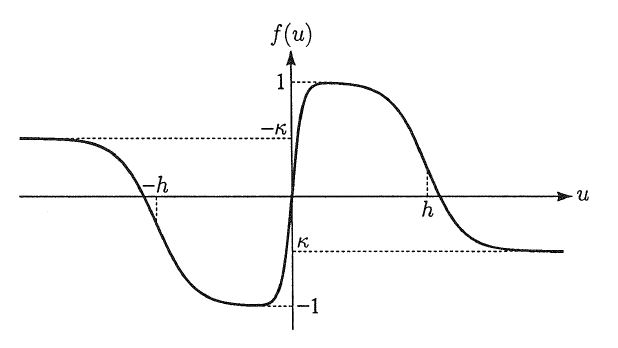
\includegraphics[scale = 0.8]{inc/nonmonotonic.jpg}
	\caption{The nonmonotonic output function, S.Yoshizawa, M.Morita and S.Amari(1992)}
	\label{fig:nonmonotonic}
\end{figure}

%THIS IS STH EXTRA OUTSIDE HOPFIELD
\subsection{Experiment on Implicit Memory for Novel Associations between pictures: \\ Effects of Stimulus Unitization and Aging\cite{stimulus_unitization_and_aging}}

From various previous research, concepts such as associative priming, unitization, difference between conceptual and perceptual associative priming, verbal versus pictorial material/stimuli and roll of spatial proximity were briefly summarized.

Experiments with pictorial stimuli(paired pictures) were done in 3 consecutive stages, where the result from first stage showed no evidence on requirement of spatial contiguity, though associative priming was enhanced compared to with spatially separated stimuli, which proved "implicit memory for novel associations still can occur in the absence of an emergent conceptual representation". The second experiment was an extension from the first experiment, with focus on the effects of aging and spatial contiguity of the same topic of stimuli on novel association priming between pictures, where stunning result was shown that "associative priming is age invariant"(exposure of pictures was longer with older group to yield a matched performance in the baseline). The last experiment was based on both first and second experiments that "associative priming with pictorial stimuli is modulated by spatial contiguity but not by aging", and the study proved further evidence for the notion that novel association priming for picture pairs is mediated by the PRS(Perceptual Representation System).

TODO: Move applications and capabilities of Hopfields from the Model section to this section.

%Wenting.

%1982, $0.15n$ (capacity of associative memory)
%
%% Above 0.15n releases the constraint on symmetries according to Olle.
%
%1985, proven $ \frac{n}{2\log{n}} $ (absolute capacity)
%
%1985, $0.14n$ (relative capacity of recalling process)
%
%1993, $ n ~= 0.4n $ (new result, absolute capacity)
